% ======================================================================
% Přednáška 2 (OneNote: \uv{1. Prednaska, 2.cast}, pokračování, 10. 10. 2022)
% Rutherfordův vzorec, kvantový popis rozptylu, nerozlišitelnost, formfaktor
% ======================================================================
\section{Rutherfordův vzorec, kvantový popis rozptylu a formfaktor}

Původní poznámky k této přednášce (\texttt{prednaska\_02.pdf}) začínají celou látkou předchozí části -- rozptylem tvrdých koulí a začátkem klasického odvození Rutherfordova rozptylu. Úseky P02-1 a P02-2 jsou shodné s P01-1 a P01-2 (a začátek P02-3 s P01-3), proto je zde neopakujeme a odkazujeme na předchozí kapitolu. Navážeme přesně tam, kde jsme skončili: u integrálu $(*)$ pro změnu hybnosti.

\subsection{Dokončení klasického odvození}

\strana{P02-3}
Připomeňme, kde jsme: změnu hybnosti $\Delta p = 2p\sin\frac{\theta}{2}$ jsme vyjádřili jako integrál průmětu Coulombovy síly přes úhel $\varphi$ a úhlovou rychlost jsme nahradili ze zákona zachování momentu hybnosti, $\omega = v_0 b/r^2$. Neznámá funkce $r(\varphi)$ se tím pokrátila a integrál je triviální:
\begin{equation}
  (*)\qquad 2p\sin\frac{\theta}{2}
  = \int_{-\frac{\pi-\theta}{2}}^{\frac{\pi-\theta}{2}}
    \underbrace{\frac{qQe^2}{4\pi\varepsilon_0}\,\frac{1}{r^2(\varphi)}}_{F(\varphi)}\cos\varphi\,\frac{r^2(\varphi)}{v_0 b}\,\dd\varphi
  = \frac{qQe^2}{4\pi\varepsilon_0}\,\frac{1}{v_0 b}\Big[\sin\varphi\Big]_{-\frac{\pi-\theta}{2}}^{\frac{\pi-\theta}{2}}
  = \frac{qQe^2}{4\pi\varepsilon_0}\,\frac{1}{v_0 b}\,2\cos\frac{\theta}{2},
\end{equation}
kde jsme využili $\sin\frac{\pi-\theta}{2} = \cos\frac{\theta}{2}$. Na levé straně dosadíme $p = m v_0$:
\begin{equation}
  2 m v_0 \sin\frac{\theta}{2} = \frac{qQe^2}{4\pi\varepsilon_0}\,\frac{1}{v_0 b}\,2\cos\frac{\theta}{2}
\end{equation}
a vyjádříme záměrný parametr jako funkci úhlu rozptylu -- to je coulombovská obdoba vztahu $b=(r_1+r_2)\cos\frac{\theta}{2}$ pro tvrdé koule:
\begin{equation}
  \vzorec{b = \frac{qQe^2}{4\pi\varepsilon_0}\,\frac{1}{m v_0^2}\,\operatorname{cotg}\frac{\theta}{2}}
\end{equation}
Fyzikálně: čím blíž částice proletí kolem jádra (menší $b$) a čím je pomalejší (menší $m v_0^2 = 2T$), tím víc se odchýlí. Veličina $\frac{qQe^2}{4\pi\varepsilon_0 m v_0^2}$ má rozměr délky; je to polovina vzdálenosti nejtěsnějšího přiblížení při čelní srážce (viz níže).

\paragraph{Diferenciální účinný průřez.}
Teď použijeme přesně stejný recept jako u tvrdých koulí. K derivaci potřebujeme $(\operatorname{cotg} x)' = -\frac{1}{\sin^2 x}$, takže $\dd b = \frac{qQe^2}{4\pi\varepsilon_0 m v_0^2}\,(-1)\frac{1}{\sin^2\frac{\theta}{2}}\,\frac{\dd\theta}{2}$:
\begin{equation}
  \dv{\sigma}{\Omega} = \frac{2\pi b\,\dd b}{2\pi\sin\theta\,\dd\theta}
  = \left(\frac{qQe^2}{4\pi\varepsilon_0 m v_0^2}\right)^2
    \frac{\operatorname{cotg}\frac{\theta}{2}\,(-1)\,\frac12}{\sin\theta\,\sin^2\frac{\theta}{2}} .
\end{equation}
Po dosazení $\sin\theta = 2\sin\frac{\theta}{2}\cos\frac{\theta}{2}$ a vzetí absolutní hodnoty dostáváme \kw{Rutherfordův vzorec}:
\begin{veta}[Rutherfordův vzorec]
\begin{equation}
  \vzorec{\dv{\sigma}{\Omega} = \left(\frac{qQe^2}{8\pi\varepsilon_0\, m v_0^2}\right)^2 \frac{1}{\sin^4\frac{\theta}{2}}}
\end{equation}
\end{veta}
Charakteristická závislost $\sin^{-4}(\theta/2)$ je \uv{otisk prstu} \emph{bodového} coulombovského centra. Rutherfordova měření úhlového rozdělení $\alpha$ částic na zlaté fólii s ní souhlasila přes mnoho řádů -- z toho plyne, že kladný náboj atomu je soustředěn v objektu mnohem menším, než je atom (viz Davídkovy slajdy, \uv{Rutherfordův experiment (2)}). V proměnných ze cvičení ($q=Z_1$, $Q=Z_2$, $T_0 = \frac12 m v_0^2$, $\frac{e^2}{4\pi\varepsilon_0} = \alpha\hbar c$) je to $\dv*{\sigma}{\Omega} = \left(\frac{\alpha\hbar c Z_1Z_2}{4T_0}\right)^2\sin^{-4}\frac{\theta}{2}$.

\paragraph{Účinný průřez pro rozptyl nad daný úhel.}
Experimentálně často počítáme všechny částice rozptýlené o víc než nějaký úhel $\theta_0$. Integrujeme přes prostorový úhel $\dd\Omega = 2\pi\sin\theta\,\dd\theta$ a zase píšeme $\sin\theta = 2\sin\frac\theta2\cos\frac\theta2$, $\dd\theta = 2\,\dd\frac{\theta}{2}$:
\begin{equation}
  \sigma(\theta>\theta_0) = \int_{\theta_0}^{\pi}\dv{\sigma}{\Omega}\,2\pi\sin\theta\,\dd\theta
  = 2\pi(\ldots)^2\int_{\theta_0}^{\pi}\frac{1}{\sin^4\frac{\theta}{2}}\,2\sin\frac{\theta}{2}\cos\frac{\theta}{2}\,2\,\dd\frac{\theta}{2} =
\end{equation}

\strana{P02-4}
Substitucí $\xi = \sin\frac{\theta}{2}$, $\dd\xi = \cos\frac{\theta}{2}\,\dd\frac{\theta}{2}$ (meze $\sin\frac{\theta_0}{2}$ až $1$):
\begin{equation}
  = 8\pi(\ldots)^2\int_{\sin\frac{\theta_0}{2}}^{1}\frac{1}{\xi^3}\,\dd\xi
  = 4\pi\left(\frac{qQe^2}{8\pi\varepsilon_0 m v_0^2}\right)^2\operatorname{cotg}^2\frac{\theta_0}{2},
\end{equation}
neboť $\int_s^1\xi^{-3}\dd\xi = \frac{1}{2s^2}-\frac12 = \frac{1-s^2}{2s^2} = \frac12\operatorname{cotg}^2\frac{\theta_0}{2}$.

\pozor{Pro $\theta_0\to0$ tento průřez diverguje} -- celkový Rutherfordův účinný průřez je nekonečný. Důvodem je nekonečný dosah Coulombova potenciálu: i částice s obrovským $b$ se trochu odchýlí. Ve skutečnosti je jádro v atomu odstíněno elektrony, takže pro velmi malé úhly (velká $b$, srovnatelná s rozměrem atomu) Rutherfordův vzorec neplatí.

\subsection{Nejmenší vzdálenost přiblížení}

\emph{Kdy se dostanu nejblíž?} Rutherfordův vzorec předpokládá bodové jádro. Platí tedy jen tak dlouho, dokud se částice nedostane tak blízko, že by \uv{ucítila} konečný rozměr jádra (a jaderné síly). Nejblíž se dostane při čelní srážce ($b=0$): celá kinetická energie se v bodě obratu přemění na potenciální energii,
\begin{equation}
  T = \frac12 m v_0^2 = \frac{qQe^2}{4\pi\varepsilon_0\,r_{\min}} .
\end{equation}
Pro numerický odhad je výhodné vytknout bezrozměrnou \kw{konstantu jemné struktury} $\alpha = \frac{e^2}{4\pi\varepsilon_0\hbar c}\approx\frac{1}{137}$ a použít $\hbar c \approx 197\ \mathrm{MeV\cdot fm}$:
\begin{equation}
  r_{\min} = \frac{qQe^2}{e^2}\,\underbrace{\frac{e^2}{4\pi\varepsilon_0\hbar c}}_{\alpha}\,\frac{\hbar c}{T}
  = q\cdot Q\,\frac{1}{137}\,\frac{197\ \mathrm{fm\cdot MeV}}{T} .
\end{equation}

\begin{priklad}[Částice $\alpha$ na zlatě]
Pro $\alpha$ částici ($q=2$) z rozpadu $^{214}$Po o energii $T_\alpha = 7{,}7\ \mathrm{MeV}$ a jádro zlata ($Q=79$):
\[
  r_{\min} = \frac{2\cdot 79}{137}\cdot\frac{197\ \mathrm{MeV\,fm}}{7{,}7\ \mathrm{MeV}} \approx 1{,}15\cdot 25{,}6\ \mathrm{fm}
  \quad\Longrightarrow\quad r_{\min}\approx 30\ \mathrm{fm}.
\]
Poloměr jádra zlata je $R\approx 1{,}2\,A^{1/3}\ \mathrm{fm}\approx 7\ \mathrm{fm}$, tedy $r_{\min}>R$: částice se k jádru nikdy nedostane natolik, aby cítila jeho strukturu nebo jaderné síly, a proto Rutherfordovi vyšel čistý coulombovský rozptyl na \uv{bodu}. Odchylky od Rutherfordova vzorce (a tím informaci o velikosti jádra) dostaneme až při vyšších energiích nebo lehčích terčích.
\end{priklad}

\subsection{Kvantový popis (QM)}

Klasické odvození pracuje s trajektoriemi, které v mikrosvětě nemají smysl. Ukážeme, jak se účinný průřez definuje kvantově, a uvidíme, že pro Coulombův potenciál dostaneme -- náhodou -- přesně stejný výsledek. Kvantový formalismus je ale nutný pro další kroky: interferenci u nerozlišitelných částic a formfaktor.

Daleko od terče hledáme stacionární řešení ve tvaru dopadající \kw{rovinné vlny} plus rozptýlené \kw{kulové vlny}:
\begin{equation}
  \psi(x) = \frac{1}{(2\pi\hbar)^{3/2}}\Big[\underbrace{e^{i\vec k\cdot\vec x}}_{\text{rovinná vlna}} + \underbrace{f(\vec p',\vec p)\,\frac{e^{ikr}}{r}}_{\text{kulová vlna}}\Big],
  \qquad \hbar\vec k = \vec p .
\end{equation}
Zde $\vec p$ je hybnost dopadající částice, $\vec p'$ hybnost rozptýlené částice (stejné velikosti, ve směru pozorování) a $f(\vec p',\vec p)$ je \kw{amplituda rozptylu} -- veškerá fyzika interakce je schována v ní. Faktor $1/r$ zajišťuje, že tok kulovou vlnou plochou $r^2\dd\Omega$ nezávisí na $r$ (zachování počtu částic).

Účinný průřez opět definujeme jako poměr toku rozptýlených částic plochou $\dd\vec S$ k hustotě dopadajícího toku:
\begin{equation}
  \dd\sigma = \frac{\vec j_{\mathrm{out}}\cdot\dd\vec S}{|\vec j_{\mathrm{in}}|},
  \qquad
  \vec j = \frac{-i\hbar}{2m}\left(\psi^*\vec\nabla\psi - \psi\vec\nabla\psi^*\right),
\end{equation}
kde $\vec j$ je \kw{hustota toku pravděpodobnosti} (odvodíme ji za chvíli). Pro rovinnou vlnu $e^{ikz}$ (osu $z$ volíme ve směru svazku; společný normalizační faktor se v poměru pokrátí):

\strana{P02-5}
\begin{equation}
  |\vec j_{\mathrm{in}}| = \frac{-i\hbar}{2m}\left[e^{-ikz}\,ik\,e^{ikz} - e^{ikz}(-ik)\,e^{-ikz}\right] = \frac{\hbar k}{m} = \frac{p}{m},
\end{equation}
což je prostě rychlost -- hustota toku jedné částice v jednotkovém objemu. Pro kulovou vlnu (ve velké vzdálenosti, kde přežívá jen derivace exponenciály) a pro element plochy koule:
\begin{equation}
  \left.
  \begin{aligned}
    \vec j_{\mathrm{out}} &= \frac{p}{m}\,|f(\vec p',\vec p)|^2\,\frac{1}{r^2}\,\frac{\vec r}{|\vec r|}\\
    \dd\vec S &= r^2\,\dd\Omega\,\frac{\vec r}{|\vec r|}
  \end{aligned}
  \right\}
  \quad\Longrightarrow\quad
  \vzorec{\dv{\sigma}{\Omega} = |f(\vec p',\vec p)|^2}
\end{equation}
Diferenciální účinný průřez je kvadrát absolutní hodnoty amplitudy rozptylu. (Interferenci rovinné a kulové vlny zanedbáváme -- detektor mimo osu svazku dopadající vlnu \uv{nevidí}.)

\subsubsection*{Odvození hustoty toku ze Schrödingerovy rovnice}
Výraz pro $\vec j$ není libovolný: plyne ze \kw{zachování pravděpodobnosti}. Vyjdeme ze \kw{Schrödingerovy rovnice} a její komplexně sdružené verze. První vynásobíme $(-i\psi^*)$, druhou $(i\psi)$:
\begin{align}
  i\hbar\pdv{\psi}{t} &= \frac{-\hbar^2}{2m}\Delta\psi + V\psi \qquad \Big/\cdot(-i\psi^*)
  &&\Longrightarrow\quad \hbar\psi^*\pdv{\psi}{t} = \frac{i\hbar^2}{2m}\psi^*\Delta\psi - iV\psi^*\psi \\
  -i\hbar\pdv{\psi^*}{t} &= \frac{-\hbar^2}{2m}\Delta\psi^* + V\psi^* \qquad \Big/\cdot(i\psi)
  &&\Longrightarrow\quad \hbar\psi\pdv{\psi^*}{t} = \frac{-i\hbar^2}{2m}\psi\Delta\psi^* + iV\psi^*\psi
\end{align}
\pozn{u této části je v originále na pravém okraji zakroužkované \uv{4} -- patrně číslo strany/odkazu}
Sečtením se potenciálové členy (pro reálné $V$) vyruší:
\begin{align}
  \hbar\left[\psi^*\pdv{\psi}{t} + \psi\pdv{\psi^*}{t}\right] &= \frac{i\hbar^2}{2m}\left[\psi^*\Delta\psi - \psi\Delta\psi^*\right],\\
  \pdv{t}\underbrace{|\psi|^2}_{\rho} &= \frac{i\hbar}{2m}\left[\psi^*\Delta\psi - \psi\Delta\psi^*\right].
\end{align}
Pravou stranu lze napsat jako divergenci, protože $\vec\nabla\cdot(\psi^*\vec\nabla\psi - \psi\vec\nabla\psi^*) = \psi^*\Delta\psi - \psi\Delta\psi^*$ (smíšené členy $\vec\nabla\psi^*\cdot\vec\nabla\psi$ se odečtou). Porovnáním s \kw{rovnicí kontinuity}
\begin{equation}
  \pdv{\rho}{t} + \div\vec j = 0
  \qquad\Longrightarrow\qquad
  \vzorec{\vec j = \frac{-i\hbar}{2m}\left[\psi^*\vec\nabla\psi - \psi\vec\nabla\psi^*\right]}
\end{equation}
Úbytek pravděpodobnosti v objemu je tedy roven toku $\vec j$ jeho hranicí -- přesně ve smyslu, v jakém jsme $\vec j$ použili k počítání částic prolétajících plochou detektoru.

\subsection{Lippmannova--Schwingerova rovnice a Bornova aproximace}

\strana{P02-6}
Zbývá spočítat amplitudu $f$ pro daný potenciál. Schrödingerovu rovnici s okrajovou podmínkou \uv{rovinná vlna + odcházející kulová vlna} lze přepsat do integrálního tvaru: vlnová funkce $\psi(\vec x)$ splňuje tzv.\ \kw{Lippmannovu--\allowbreak Schwingerovu rovnici}. V asymptotické oblasti ($r\to\infty$) a v nejnižším řádu v potenciálu (tj. v \kw{první Bornově aproximaci}, kde pod integrál místo přesného $\psi$ dosadíme nerozptýlenou vlnu $\psi_0$) má tvar
\begin{equation}
  \psi(\vec x) = \psi_0(\vec x) + \left[\frac{-2m}{4\pi\hbar^2}\int e^{-i\vec k'\cdot\vec x'}\,V(\vec x')\,\psi_0(\vec x')\,\dd^3\vec x'\right]\frac{e^{ikr}}{r},
\end{equation}
kde
\[
  \psi_0(\vec x) = \frac{1}{\oprava{(2\pi\hbar)^{3/2}}{(2\pi\hbar^2)^{3/2}}}\,e^{i\vec k\cdot\vec x},
  \qquad
  [\ \ldots\ ] = \frac{1}{(2\pi\hbar)^{3/2}}\,f(\vec k',\vec k) .
\]
(Normalizace musí být stejná jako ve vzorci pro $\psi(x)$ výše; v poznámkách je zde i v části o formfaktoru $\hbar^2$, na výsledcích to ale nic nemění, protože se pokrátí.) Porovnáním tedy
\begin{equation}
  \vzorec{f(\vec k',\vec k) = \frac{-2m}{4\pi\hbar^2}\int e^{-i\vec k'\cdot\vec x'}\,V(\vec x')\,e^{i\vec k\cdot\vec x'}\,\dd^3\vec x'}
\end{equation}
Amplituda rozptylu je v Bornově aproximaci (až na konstantu) \kw{Fourierova transformace potenciálu} v přenesené hybnosti. To je velmi silný výsledek: měřením úhlového rozdělení \uv{vidíme} Fourierův obraz potenciálu.

\begin{vysvetleni}[Odkud se bere kulová vlna]
Schrödingerovu rovnici přepíšeme jako $(\Delta + k^2)\psi = \frac{2m}{\hbar^2}V\psi$. Greenova funkce operátoru $\Delta+k^2$ s odcházející kulovou vlnou je $G(\vec x,\vec x') = -\frac{1}{4\pi}\frac{e^{ik|\vec x-\vec x'|}}{|\vec x-\vec x'|}$, takže $\psi = \psi_0 + \frac{2m}{\hbar^2}\int G\,V\psi\,\dd^3x'$ (to je přesná Lippmannova--Schwingerova rovnice). Daleko od terče rozvineme $k|\vec x-\vec x'| \approx kr - \vec k'\cdot\vec x'$ (přesně tento rozvoj uděláme níže u formfaktoru) a dostaneme hranatou závorku výše. Bornova aproximace $\psi\to\psi_0$ pod integrálem je oprávněná, když je potenciál \uv{slabý} vůči kinetické energii.
\end{vysvetleni}

\paragraph{Yukawův potenciál.}
Spočteme amplitudu pro \kw{Yukawův (stíněný Coulombův) potenciál}
\begin{equation}
  V = V_0\,\frac{e^{-\mu r}}{r},\qquad \mu>0 .
\end{equation}
Parametr $\mu$ udává dosah ($1/\mu$); důvod, proč nezačneme rovnou Coulombem, je ten, že Fourierův integrál čistého $1/r$ nekonverguje -- regularizujeme ho faktorem $e^{-\mu r}$ a na konci pošleme $\mu\to0$. (Fyzikálně to navíc odpovídá stínění jádra elektronovým obalem.) Pro integrál ve vzorci pro $f$:
\begin{equation}
  \int e^{-i\vec k'\cdot\vec x'}\,\frac{e^{-\mu r}}{r}\,e^{i\vec k\cdot\vec x'}\,\dd^3x' \;\longrightarrow\; \int e^{iqr\cos\theta}\,\frac{e^{-\mu r}}{r}\,\dd^3x,
\end{equation}
kde $\vec q = \vec k - \vec k'$ \pozn{v poznámkách vpravo $\vec q = (\vec p-\vec p')/\hbar$; dále u formfaktoru opačné znaménko $\hbar\vec q = \vec p'-\vec p$ -- na $|\vec q|$ to nemá vliv} a osu $z$ sférických souřadnic jsme zvolili ve směru $\vec q$. Substituce
\[
  iqr\cos\theta = \xi,\qquad -iqr\sin\theta\,\dd\theta = \dd\xi
\]
dává (integrace přes azimut dá $2\pi$, meze $\theta=0\mapsto\xi=iqr$, $\theta=\pi\mapsto\xi=-iqr$):
\begin{equation}
  2\pi\int_0^\infty r^2\dd r\int_{+iqr}^{-iqr}\frac{\dd\xi}{-iqr}\,e^{\xi}\,\frac{e^{-\mu r}}{r}
  = \oprava{\frac{4\pi}{q}}{\frac{4\pi}{q^2}}\int_0^\infty \dd r\,\sin(qr)\,e^{-\mu r},
\end{equation}
protože vnitřní integrál je $\frac{e^{-iqr}-e^{iqr}}{-iqr} = \frac{2\sin(qr)}{qr}$. (Další řádek v poznámkách už správně počítá s $\frac{4\pi}{q}$.) Odtud
\begin{align}
  f &= \frac{-2m}{4\pi\hbar^2 q}\,V_0\int_0^\infty\sin(qr)\,e^{-\mu r}\,\dd r\;4\pi
     = \frac{-2m}{\hbar^2 q}\,V_0\int_0^\infty \operatorname{Im}\left(e^{iqr-\mu r}\right)\dd r = \\
    &= \frac{-2m}{\hbar^2 q}\,V_0\operatorname{Im}\left[\frac{e^{(iq-\mu)r}}{iq-\mu}\right]_0^\infty
     = \frac{2m}{\hbar^2 q}\,V_0\operatorname{Im}\left(\frac{1}{iq-\mu}\right) = \\
    &= \frac{-2m}{\hbar^2 q}\,V_0\operatorname{Im}\left(\frac{iq+\mu}{q^2+\mu^2}\right)
     = \frac{-2m}{\hbar^2}\,V_0\,\frac{1}{q^2+\mu^2}.
\end{align}
Horní mez je nulová díky $\mu>0$ (exponenciála utlumí oscilace) -- tady regularizace skutečně pracuje. Ve třetím řádku jsme rozšířili zlomek: $\frac{1}{iq-\mu} = -\frac{iq+\mu}{q^2+\mu^2}$.

\strana{P02-7}
Velikost přenesené hybnosti souvisí s úhlem rozptylu: $\vec p$ a $\vec p'$ mají stejnou velikost $p$ a svírají úhel $\theta$, takže (stejný rovnoramenný trojúhelník jako v klasickém odvození)
\[
  \vec q = \frac{\vec p-\vec p'}{\hbar},\qquad \frac{\hbar q}{2p} = \sin\frac{\theta}{2}.
\]

\paragraph{Limita $\mu\to0$: Coulombův potenciál.} Položíme $V_0 = \frac{qQe^2}{4\pi\varepsilon_0}$ (v poznámkách pro jednotkové náboje, $V_0=\frac{e^2}{4\pi\varepsilon_0}$; pozor, $q$ zde označuje přenesenou hybnost, nikoli náboj) a $q^2 = \frac{4p^2}{\hbar^2}\sin^2\frac\theta2 = \frac{4m^2v_0^2}{\hbar^2}\sin^2\frac\theta2$:
\begin{equation}
  f = \frac{-2m}{\hbar^2}\,V_0\,\frac{1}{q^2} = -\frac{e^2}{8\pi\varepsilon_0\,m v_0^2}\,\frac{1}{\sin^2\frac{\theta}{2}},
  \qquad
  \dv{\sigma}{\Omega} = |f|^2 .
\end{equation}
\pozn{v poznámkách bez znaménka minus -- pro $\dv*{\sigma}{\Omega}=|f|^2$ nepodstatné}
Kvadrát $|f|^2$ je \emph{přesně} klasický Rutherfordův vzorec, i když jsme použili jen první Bornovu aproximaci. To je zvláštní \uv{šťastná náhoda} Coulombova potenciálu (přesné kvantové řešení se od Bornova liší jen fází amplitudy) -- a je to důvod, proč Rutherford mohl s klasickou fyzikou dostat správný výsledek.

\begin{vysvetleni}[Proč je amplituda $\propto 1/q^2$]
Výsledek $f\propto V_0/(q^2+\mu^2)$ je Fourierův obraz Yukawova potenciálu. V jazyce kvantové teorie pole odpovídá výměně částice s hmotností $\mu$ (v jednotkách $\hbar=c=1$) -- tzv. \kw{propagátor} $1/(q^2+\mu^2)$. Yukawa tak v roce 1935 z dosahu jaderných sil ($\sim 1{,}4$ fm) předpověděl pion s hmotností $\approx 140\ \mathrm{MeV}$. Pro foton ($\mu=0$) dostáváme $1/q^2$, tedy coulombovský rozptyl s nekonečným dosahem a divergencí při $q\to 0$.
\end{vysvetleni}

\subsection{Nerozlišitelnost částic}

Rozptylují-li se na sobě dvě \kw{stejné částice} (např. dva elektrony, nebo $\alpha$ na $^4$He), nemůžeme rozlišit, zda detektor pod úhlem $\theta$ (v těžišťové soustavě) zaznamenal projektil rozptýlený o $\theta$, nebo terčovou částici, která odletěla pod tímto úhlem, zatímco projektil se rozptýlil o $\pi-\theta$:

\begin{center}
\begin{tikzpicture}[scale=0.9]
  % první situace
  \draw (-2.4,0) -- (0,0);
  \draw (0,0.1) -- (1.2,0.0);
  \draw[->] (0,0.1) -- (1.3,1.0);
  \draw[->] (0,0.05) -- (-1.4,-1.0);
  \draw (0.6,0.05) arc (0:35:0.6);
  \node at (0.85,0.3) {\small $\theta$};
  \node at (2.2,0) {$\equiv$};
  % druhá situace: projektil letí dozadu (pi-theta), terč pod theta
  \draw (3.2,0.2) -- (4.9,0.2);
  \draw[->] (4.9,0.2) -- (3.6,-0.8);
  \draw (5.1,0.0) -- (6.9,0.0);
  \draw[->] (5.1,0.0) -- (6.5,1.0);
  \draw (5.75,0.0) arc (0:35:0.65);
  \node at (6.05,0.27) {\small $\theta$};
\end{tikzpicture}
\end{center}

Kvantově se pak nesčítají pravděpodobnosti, ale \emph{amplitudy} obou možností, se znaménkem daným symetrií prostorové vlnové funkce:
\begin{equation}
  f(\theta)\;\longrightarrow\; f(\theta)\pm f(\pi-\theta).
\end{equation}
Znaménko $+$ platí pro prostorově symetrickou, $-$ pro antisymetrickou vlnovou funkci.

\paragraph{Dva elektrony.} Elektrony jsou fermiony, celková vlnová funkce (prostor $\times$ spin) musí být antisymetrická. Spinové stavy dvou elektronů:
\begin{align*}
  S=0:&\quad \tfrac{1}{\sqrt2}(\uparrow\downarrow-\downarrow\uparrow) &&\text{(singlet, spinově antisymetrický $\Rightarrow$ prostorově symetrický)},\\
  S=1:&\quad \uparrow\uparrow,\ \downarrow\downarrow,\ \tfrac{1}{\sqrt2}(\uparrow\downarrow+\downarrow\uparrow) &&\text{(triplet, spinově symetrický $\Rightarrow$ prostorově antisymetrický)}.
\end{align*}
Pro nepolarizovaný svazek i terč je každý ze čtyř spinových stavů stejně pravděpodobný, tedy singlet má váhu $\frac14$ a triplet $\frac34$:
\begin{equation}
  \dv{\sigma}{\Omega} = \frac14\underbrace{\left(\dv{\sigma}{\Omega}\right)_{S=0}}_{f(\theta)+f(\pi-\theta)} + \frac34\underbrace{\left(\dv{\sigma}{\Omega}\right)_{S=1}}_{f(\theta)-f(\pi-\theta)}
\end{equation}
\begin{equation}
  \longrightarrow\ \frac14\left|f(\theta)+f(\pi-\theta)\right|^2 + \frac34\left|f(\theta)-f(\pi-\theta)\right|^2 =
\end{equation}
Dosadíme coulombovskou amplitudu $f(\theta)\propto\frac{1}{\sin^2\frac\theta2}$, tedy $f(\pi-\theta)\propto\frac{1}{\cos^2\frac\theta2}$ (společný prefaktor $\frac{e^2}{8\pi\varepsilon_0 m v_0^2}$ zatím vynecháme):

\strana{P02-8}
\begin{align}
  &= \frac14\left|\frac{1}{\sin^2\frac\theta2} + \frac{1}{\cos^2\frac\theta2}\right|^2 + \frac34\left|\frac{1}{\sin^2\frac\theta2} - \frac{1}{\cos^2\frac\theta2}\right|^2 = \\
  &= \frac{1}{4\left(\sin^2\frac\theta2\cos^2\frac\theta2\right)^2}\left[\left|\cos^2\frac\theta2+\sin^2\frac\theta2\right|^2 + 3\left|\cos^2\frac\theta2-\sin^2\frac\theta2\right|^2\right] = \\
  &= \frac{4}{\sin^4\theta}\left[1+3\cos^2\theta\right] = \frac{4}{\sin^4\theta}\left(4-3\sin^2\theta\right),
\end{align}
kde jsme použili $\sin\frac\theta2\cos\frac\theta2 = \frac12\sin\theta$ a $\cos^2\frac\theta2-\sin^2\frac\theta2 = \cos\theta$. Po vrácení prefaktoru:
\begin{equation}
  \vzorec{\dv{\sigma}{\Omega} = \left(\frac{e^2}{4\pi\varepsilon_0 m}\right)^2\frac{1}{v_0^4\sin^4\theta}\left(4-3\sin^2\theta\right) = \left(\frac{\alpha}{m}\right)^2\frac{1}{v_0^4\sin^4\theta}\left(4-3\sin^2\theta\right)}
\end{equation}
(poslední tvar v přirozených jednotkách $\hbar=c=1$, kde $\frac{e^2}{4\pi\varepsilon_0}=\alpha$).

\begin{vysvetleni}[Co je na výsledku \uv{kvantového}]
Kdyby elektrony byly rozlišitelné klasické částice, sečetli bychom jen pravděpodobnosti: $|f(\theta)|^2+|f(\pi-\theta)|^2 \propto \frac{1}{\sin^4\frac\theta2}+\frac{1}{\cos^4\frac\theta2}$. Spinově středovaný kvantový výsledek je
\[
  \tfrac14|A+B|^2+\tfrac34|A-B|^2 = A^2+B^2 - AB,\qquad A = \tfrac{1}{\sin^2\frac\theta2},\ B=\tfrac{1}{\cos^2\frac\theta2},
\]
tj. obsahuje navíc \kw{interferenční (výměnný) člen} $-AB$, který nejvíce sníží průřez kolem $\theta=90^\circ$. Je to nerelativistická \kw{Mottova formule} pro rozptyl $e^-e^-$. Při jejím použití je $\theta$ úhel v těžišťové soustavě, $v_0$ relativní rychlost a $m$ je redukovaná hmotnost soustavy (pro dva elektrony $m_e/2$) -- tak je to i u Rutherfordova vzorce, který jsme odvodili pro nepohyblivý terč.
\end{vysvetleni}

\begin{center}
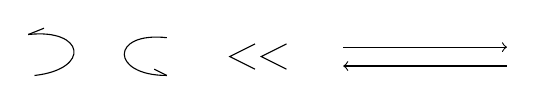
\begin{tikzpicture}[scale=0.8]
  % náčrtek z poznámek (význam nejistý)
  \draw (0,0.35) .. controls (0.9,0.45) and (1.0,-0.2) .. (0.1,-0.3);
  \draw (0,0.35) -- (0.25,0.45);
  \draw (2.2,0.3) .. controls (1.3,0.4) and (1.3,-0.3) .. (2.2,-0.3);
  \draw (2.0,-0.2) -- (2.2,-0.3);
  \draw (3.6,0.2) -- (3.2,0.0) -- (3.6,-0.2);
  \draw (4.1,0.2) -- (3.7,0.0) -- (4.1,-0.2);
  \draw[->] (5.0,0.15) -- (7.6,0.15);
  \draw[->] (7.6,-0.15) -- (5.0,-0.15);
\end{tikzpicture}
\end{center}
\pozn{v poznámkách následuje tento nejasný náčrtek ($\supset\ \subset\quad \ll\quad \rightleftarrows$); patrně znázorňuje dvě částice letící proti sobě v těžišťové soustavě, případně podmínku malých energií $\beta\ll1$ z následujícího odstavce}

\subsection{Co přinese QFT?}

V kvantové teorii pole (QED) popisujeme rozptyl dvou elektronů (\kw{Møllerův rozptyl}) Feynmanovými diagramy. Elektrony si vymění virtuální foton $\gamma$; protože jsou nerozlišitelné, přispívají dva diagramy -- \uv{přímý} ($t$-kanál) a \uv{výměnný} ($u$-kanál, koncové elektrony prohozené). Relativní znaménko $-$ mezi nimi je přesně Pauliho princip, který jsme výše zavedli ručně přes $f(\theta)\pm f(\pi-\theta)$.

\begin{center}
\begin{tikzpicture}[scale=1.0]
  % t-kanál
  \coordinate (a1) at (0,1.6); \coordinate (v1) at (1.6,1.6); \coordinate (b1) at (3.2,1.6);
  \coordinate (a2) at (0,0);   \coordinate (v2) at (1.6,0);   \coordinate (b2) at (3.2,0);
  \draw[->] (a1) -- ($(a1)!0.6!(v1)$); \draw ($(a1)!0.5!(v1)$) -- (v1);
  \draw[->] (v1) -- ($(v1)!0.6!(b1)$); \draw ($(v1)!0.5!(b1)$) -- (b1);
  \draw[->] (a2) -- ($(a2)!0.6!(v2)$); \draw ($(a2)!0.5!(v2)$) -- (v2);
  \draw[->] (v2) -- ($(v2)!0.6!(b2)$); \draw ($(v2)!0.5!(b2)$) -- (b2);
  \draw[decorate,decoration={snake,amplitude=1.5pt,segment length=6pt}] (v1) -- (v2);
  \fill (v1) circle (0.05); \fill (v2) circle (0.05);
  \node[left] at (1.5,0.8) {$\gamma$};
  \node at (4.1,0.8) {$+$};
  % u-kanál (prohozené koncové elektrony)
  \coordinate (c1) at (5.0,1.6); \coordinate (w1) at (6.6,1.6); \coordinate (d1) at (8.4,0);
  \coordinate (c2) at (5.0,0);   \coordinate (w2) at (6.6,0);   \coordinate (d2) at (8.4,1.6);
  \draw[->] (c1) -- ($(c1)!0.6!(w1)$); \draw ($(c1)!0.5!(w1)$) -- (w1);
  \draw[->] (c2) -- ($(c2)!0.6!(w2)$); \draw ($(c2)!0.5!(w2)$) -- (w2);
  \draw[->] (w1) -- (d1);
  \draw[->] (w2) -- (d2);
  \draw[decorate,decoration={snake,amplitude=1.5pt,segment length=6pt}] (w1) -- (w2);
  \fill (w1) circle (0.05); \fill (w2) circle (0.05);
  \node[left] at (6.5,0.8) {$\gamma$};
\end{tikzpicture}
\end{center}

\pozor{Vyjde to \uv{stejně}} -- pro $\beta\to0$, čili pro malé energie, se výsledek QED redukuje na výše odvozený kvantově-mechanický vzorec. Relativistické opravy (a příspěvek magnetické interakce spinů) se projeví až pro $\beta=v/c$ srovnatelné s jedničkou.

\subsection{Formfaktor}

Dosud jsme rozptylovali na \emph{bodovém} centru. Skutečná jádra (a nukleony) mají ale konečný rozměr a jejich náboj je rozložen s nějakou hustotou $\rho(\vec x)$. Ukážeme, že toto rozložení se do účinného průřezu promítne jednoduchým multiplikativním faktorem -- \kw{formfaktorem} -- a že jeho měřením lze rozložení náboje zrekonstruovat. Výchozí bod je opět asymptotická vlnová funkce
\begin{equation}
  \psi = \frac{1}{\oprava{(2\pi\hbar)^{3/2}}{(2\pi\hbar^2)^{3/2}}}\left(e^{i\vec k\cdot\vec x} + f(\vec p',\vec p)\,\frac{e^{ikr}}{r}\right),
  \qquad
  \hbar\vec q = \vec p'-\vec p,\quad \vec q = \vec k'-\vec k ,
\end{equation}
\strana{P02-9}
tentokrát pro rozptylové centrum, které \emph{není} v počátku $S$, ale v bodě $\vec x_i$. Polohu detektoru označme $\vec r$ (vůči $S$) a $\vec r_i$ (vůči centru), takže $\vec r = \vec r_i + \vec x_i$:

\begin{center}
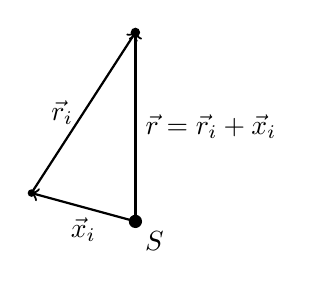
\begin{tikzpicture}[scale=1.2]
  \coordinate (S) at (0,0);
  \coordinate (X) at (-1.1,0.3);
  \coordinate (R) at (0,2);
  \fill (S) circle (0.07) node[below right] {$S$};
  \fill (X) circle (0.04);
  \fill (R) circle (0.05);
  \draw[->,thick] (S) -- (R) node[midway,right] {$\vec r = \vec r_i + \vec x_i$};
  \draw[->,thick] (S) -- (X) node[midway,below] {$\vec x_i$};
  \draw[->,thick] (X) -- (R) node[midway,left] {$\vec r_i$};
\end{tikzpicture}
\end{center}

Obě části vlnové funkce musíme vztáhnout k centru v $\vec x_i$:
\begin{itemize}[leftmargin=1.5em]
  \item rovinná vlna: $e^{i\vec k\cdot\vec x}\to e^{i\vec k\cdot\vec r_i} = e^{i\vec k\cdot(\vec r-\vec x_i)} = e^{i\vec k\cdot\vec r - i\vec k\cdot\vec x_i}$ -- jen fázový posuv;
  \item kulová vlna vychází z centra, nikoli z počátku:
  \begin{align*}
    \frac{e^{ikr}}{r}\to\frac{e^{ikr_i}}{r_i} &= \frac{e^{ik|\vec r-\vec x_i|}}{|\vec r-\vec x_i|}
    \doteq \left\{\begin{array}{l}|\vec r|\gg|\vec x_i|\\ \text{zanedbáme ve jmenovateli}\end{array}\right\}
    \doteq \frac1r\,e^{ikr\left|\frac{\vec r}{r}-\frac{\vec x_i}{r}\right|} \doteq \\
    &\doteq \frac1r\,e^{ikr\sqrt{1\,\oprava{+}{-}\,\frac{|\vec x_i|^2}{r^2}-2\frac{\vec r\cdot\vec x_i}{r^2}}} = \\
    &= \frac1r\,e^{ikr\left(1-\frac{\vec r\cdot\vec x_i}{r^2}\right)} = \frac1r\,e^{ikr - ik\frac{\vec r}{r}\cdot\vec x_i} = \frac1r\,e^{ikr-i\vec k'\cdot\vec x_i}.
  \end{align*}
\end{itemize}
Proč tyto kroky: detektor je makroskopicky daleko ($r\sim$ m) vůči rozměru terče ($x_i\sim$ fm), takže ve jmenovateli je rozdíl $r_i$ a $r$ nepodstatný. V exponentu ale nikoli -- tam se násobí velkým $k$ a malá změna dráhy způsobí konečnou změnu fáze. Proto odmocninu $|\vec r-\vec x_i| = r\sqrt{1+\frac{x_i^2}{r^2}-2\frac{\vec r\cdot\vec x_i}{r^2}}$ rozvineme do prvního řádu ($\sqrt{1+\varepsilon}\approx1+\varepsilon/2$, člen $x_i^2/r^2$ zanedbáme) -- znaménko u $|\vec x_i|^2$ je z kosinové věty $+$, na výsledek ale nemá vliv. Nakonec $k\frac{\vec r}{r} = \vec k'$ je vlnový vektor rozptýlené částice (míří k detektoru).

Celkem
\begin{align}
  \psi &= \frac{1}{(2\pi\hbar)^{3/2}}\left[e^{i\vec k\cdot\vec r - i\vec k\cdot\vec x_i} + f(\vec q)\,\frac{e^{ikr}}{r}\,e^{-i\vec k'\cdot\vec x_i}\right]
  \ \text{\uv{=}}\ \\
  \text{\uv{=}}&\ \frac{1}{(2\pi\hbar)^{3/2}}\left[e^{i\vec k\cdot\vec r} + f(\vec q)\,\frac{e^{ikr}}{r}\,e^{-i(\vec k'-\vec k)\cdot\vec x_i}\right],
\end{align}
kde \uv{$=$} znamená \uv{až na celkovou fázi $e^{-i\vec k\cdot\vec x_i}$}, kterou jsme vytkli -- celková fáze vlnové funkce je nepozorovatelná. Posunutí centra se tedy projeví jen fázovým faktorem v amplitudě:
\begin{equation}
  f(\vec q)\;\longrightarrow\; f(\vec q)\,e^{-i\vec q\cdot\vec x_i}.
\end{equation}

\strana{P02-10}
\paragraph{Když mám hodně rozptylových center} rozložených s hustotou $\rho(\vec x)$ (normovanou na jedničku), sečteme (koherentně!) amplitudy od všech center, tj. fázové faktory zintegrujeme s vahou $\rho$:
\begin{equation}
  f(\vec q)\;\longrightarrow\; f(\vec q)\cdot\underbrace{\int\rho(\vec x)\,e^{-i\vec q\cdot\vec x}\,\dd\vec x}_{F(q)\,\equiv\,\text{formfaktor}}
\end{equation}
\begin{definice}[Formfaktor]
\kw{Formfaktor} $F(\vec q)$ je Fourierova transformace (normované) hustoty rozložení náboje terče v přenesené hybnosti $\hbar\vec q$. Diferenciální účinný průřez na rozlehlém terči je
\[
  \vzorec{\dv{\sigma}{\Omega} = \left|F(\vec q)\cdot f(\vec q)\right|^2}
\]
kde $f(\vec q)$ je amplituda rozptylu na bodovém centru (např. Rutherfordova).
\end{definice}
Měříme tedy $\dv*{\sigma}{\Omega}$, vydělíme známým bodovým průřezem a dostaneme $|F(q)|^2$; zpětnou Fourierovou transformací pak (v principu) rozložení náboje $\rho(\vec x)$. Přesně tak R.~Hofstadter v 50. letech změřil velikost jader a protonu rozptylem vysokoenergetických elektronů (viz Davídkovy slajdy, \uv{Rozměr jádra}, \uv{Účinný průřez $\sigma$ (2)}).

\paragraph{1. Sféricky symetrická hustota $\rho$.} Je-li $\rho=\rho(r)$, závisí formfaktor jen na $q=|\vec q|$. Opět zvolíme osu $z$ ve směru $\vec q$:
\begin{align}
  F(q) &= \int\rho(x)\,e^{-i\vec q\cdot\vec x}\,\dd\vec x = 2\pi\int_0^\infty r^2\dd r\int_0^\pi\sin\theta\,\dd\theta\,\rho(r)\,e^{-iqr\cos\theta} = \\
       &= \frac{4\pi}{q}\int_0^\infty\rho(r)\,r\,\sin(qr)\,\dd r ,
\end{align}
(úhlový integrál je stejný jako u Yukawova potenciálu: $\int_0^\pi\sin\theta\, e^{-iqr\cos\theta}\dd\theta = \frac{2\sin(qr)}{qr}$).

Co se stane pro $q\to0$? Platí $\lim_{q\to0}\frac{1}{q}\sin(qr) = r$, takže
\[
  \lim_{q\to0}F(q) = 4\pi\int_0^\infty\rho(r)\,r^2\,\dd r = 1,
\]
díky normování $\oprava{4\pi\int_0^\infty\rho(r)\,r^2\,\dd r = 1}{\int_0^\infty\rho(r)r^2\dd r = 1}$ (tj. $\int\rho\,\dd^3x = 1$; bez faktoru $4\pi$ by limita nevyšla jedna). Fyzikálně: při malé přenesené hybnosti (dlouhé vlnové délce $\lambda\sim1/q$ vůči rozměru terče) projektil vnitřní strukturu terče \uv{nerozliší} a vidí ho jako bodový náboj -- formfaktor je jedna a platí Rutherfordův vzorec.

\begin{vysvetleni}[Rozvoj pro malá $q$: střední kvadratický poloměr]
Rozvineme-li $\sin(qr) \approx qr - \frac{(qr)^3}{6}$, dostaneme
\[
  F(q) \approx 4\pi\int_0^\infty\rho\,r^2\dd r - \frac{q^2}{6}\,4\pi\int_0^\infty\rho\,r^4\dd r = 1-\frac{q^2\langle r^2\rangle}{6}.
\]
První odchylka formfaktoru od jedničky tedy měří \kw{střední kvadratický poloměr} $\langle r^2\rangle$ rozložení náboje (viz Davídkovy slajdy, \uv{Účinný průřez $\sigma$ (2)}). Abychom rozlišili detaily o velikosti $R$, potřebujeme $q\gtrsim1/R$; pro jádra s $R\sim$ několik fm to znamená přenesené hybnosti $\hbar q\gtrsim 100$ MeV/$c$ -- proto se k měření struktury jader používají elektrony se stovkami MeV. Z takových měření plyne známý vztah $R\approx R_0A^{1/3}$, $R_0\approx1{,}2$ fm.
\end{vysvetleni}
